\section{Simple cavity}
\label{sec:simple_cavity}

We consider a slab of chiral medium characterized by periodicity $p$, average refractive index $\bar{n}$ and birefringence $\delta n$ between two isotropic media of refractive indices $n_1$ and $n_2$. Figure \ref{fig:simple_cavity} schematizes the cavity.

\subsection{Reflectivities}

To ensure the correctness of the implementation of coupled wave theory and exact theory, the reflection coefficients yielded by both methods are plotted in figure \ref{fig:simple_cavity:reflection}. The parameters used for this simulation are given in table \ref{tab:simple_cavity:reflection}. The original study took into account the angle of the plane wave in respect of $z$. Although it would be possible to do so here as well, the choice was made to only consider plane waves propagating along $\bm{z}$ axis. To fit the parameters of the previous study, $\epsilon_a$ was thus tuned to take into account the relative permittivity a plane wave propagating along another axis than $\bm{z}$.

The results given by both theories are satisfactory and approximate theory matches fairly well exact theory, with variations up to $1\%$ on the band edges. However, it can be noted that the results given in \cite{mccall_simplified_2009} are closer to exact theory than what appears in figure \ref{fig:simple_cavity:reflection}. This is because the reflection coefficients derived there use Fresnel formulas rather than the method described in section \ref{sec:interface_iso}. It appears that Fresnel coefficients are more exact. This hints that it may be possible to derive more precise matrices to switch between circular and electromagnetic bases.

\begin{table}
	\centering
	\begin{tabulary}{\linewidth}{LCC}
		\hline
		\hline
		Structural period of the chiral medium & $L_p$ & 300 nm \\
		Length of the chiral medium & $L$ & $20\times L_p$ \\
		Refractive index of the surrounding media & $n_1$ & 1 \\
		 & $n_2$ & 2 \\
		Relative permittivity $a$ & $\epsilon_a$ & $3.0897 + 0.0201i$ \\
		Relative permittivity $b$ & $\epsilon_b$ & $2.9+0.02i$ \\
		\hline
		\hline
	\end{tabulary}
	\caption[Parameters for the simple cavity]{Parameters used to calculate reflectivities. Those are equivalent to the parameters used in \cite{mccall_simplified_2009}.}
	\label{tab:simple_cavity:reflection}
\end{table}

\begin{figure}
	\centering
	\begin{subfigure}{0.32\linewidth}
		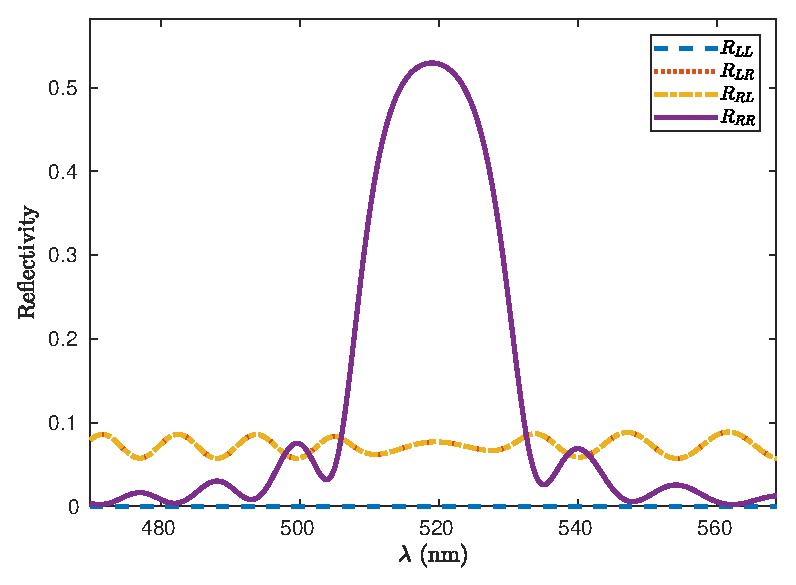
\includegraphics[width=\linewidth]{plots/simple/reflection_oseen}
		\caption{}
		\label{fig:simple_cavity:reflection_oseen}
	\end{subfigure}
	\begin{subfigure}{0.32\linewidth}
		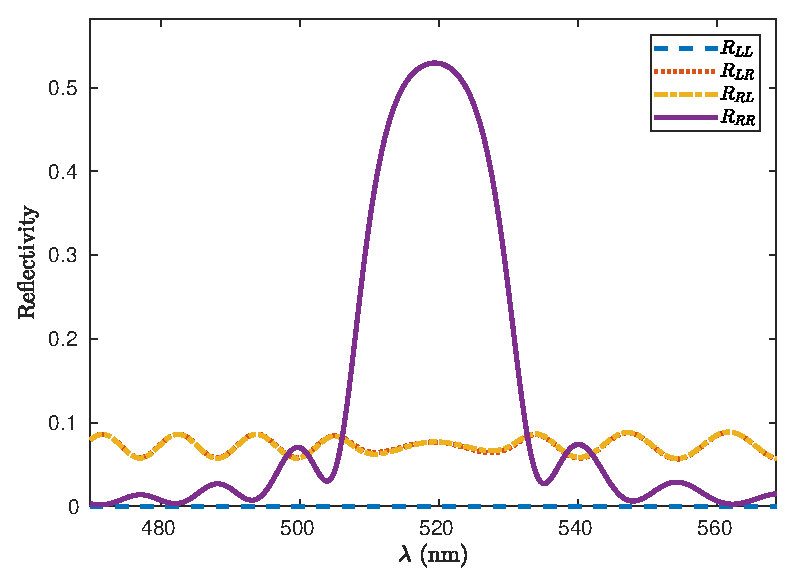
\includegraphics[width=\linewidth]{plots/simple/reflection_cwt}
		\caption{}
		\label{fig:simple_cavity:reflection_cwt}
	\end{subfigure}
	\begin{subfigure}{0.32\linewidth}
		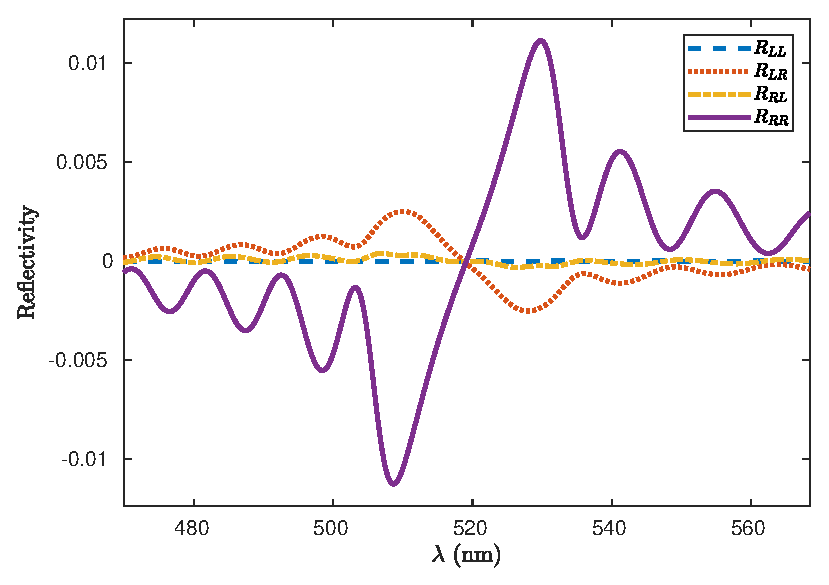
\includegraphics[width=\linewidth]{plots/simple/reflection_comp}
		\caption{}
		\label{fig:simple_cavity:reflection_comp}
	\end{subfigure}
	\begin{subfigure}{0.32\linewidth}
		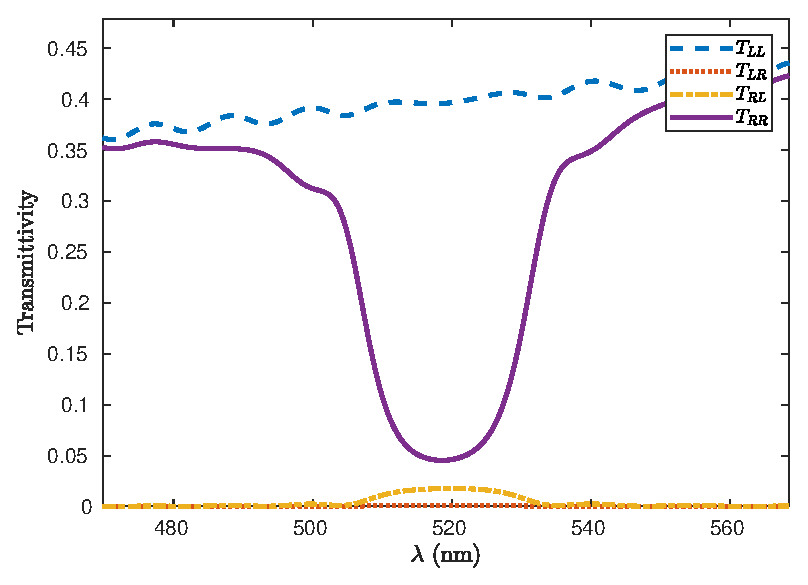
\includegraphics[width=\linewidth]{plots/simple/transmission_oseen}
		\caption{}
		\label{fig:simple_cavity:transmission_oseen}
	\end{subfigure}
	\begin{subfigure}{0.32\linewidth}
		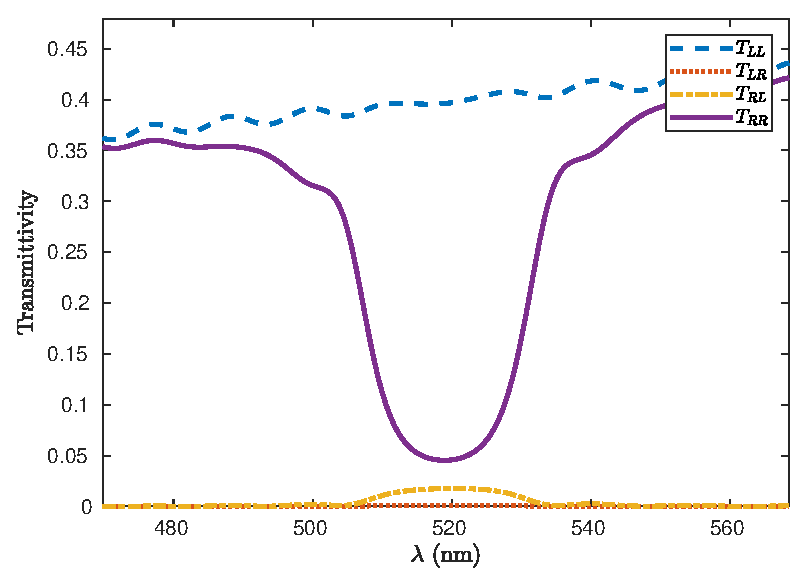
\includegraphics[width=\linewidth]{plots/simple/transmission_cwt}
		\caption{}
		\label{fig:simple_cavity:transmission_cwt}
	\end{subfigure}
	\begin{subfigure}{0.32\linewidth}
		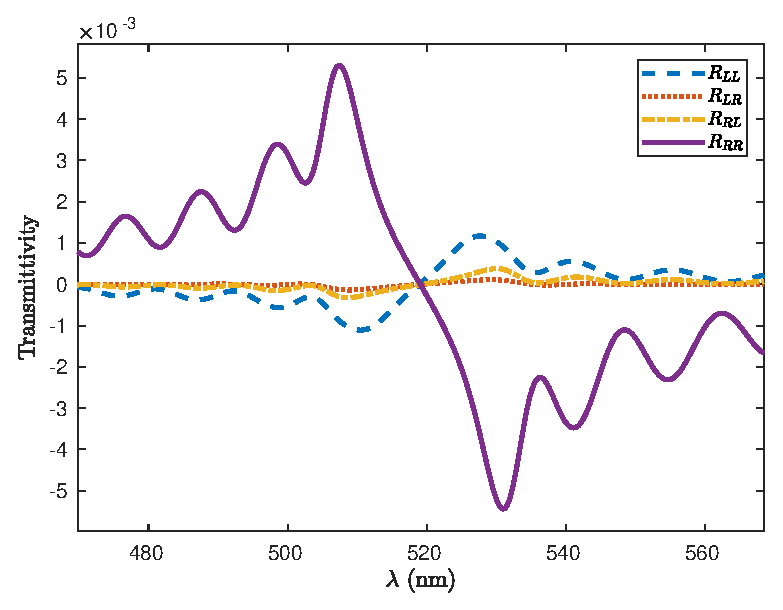
\includegraphics[width=\linewidth]{plots/simple/transmission_comp}
		\caption{}
		\label{fig:simple_cavity:transmission_comp}
	\end{subfigure}
	\caption[Comparison of reflectivities and transmittivities for a simple cavity]{Comparison of reflectivities and transmittivities for a simple cavity of right-handed medium. \ref{fig:simple_cavity:reflection_oseen} Reflectivities calculated with the Oseen method. \ref{fig:simple_cavity:reflection_cwt} Reflectivities calculated with the coupled wave theory. \ref{fig:simple_cavity:reflection_comp} Comparison of reflectivities obtained with the two methods. \ref{fig:simple_cavity:transmission_oseen} Transmittivities calculated with the Oseen method. \ref{fig:simple_cavity:transmission_cwt} Transmittivities calculated with the coupled wave theory. \ref{fig:simple_cavity:transmission_comp} Comparison of transmittivities obtained with the two methods.}
	\label{fig:simple_cavity:reflection}
\end{figure}

\subsection{Energy conservation}

The second verification made was upon energy conservation. The only comparison possible here is between exact and approximate theory. Figure \ref{fig:simple_cavity:energy_conservation} Shows the comparison of the three measures of energy conservation for both exact and approximate theories. As expected, exact theory conserves energy down to machine precision, while approximate theory ensure less precisely the conservation of energy, especially its redistribution between left and right-handed polarised light.

\begin{figure}
	\centering
	\begin{subfigure}{0.49\linewidth}
		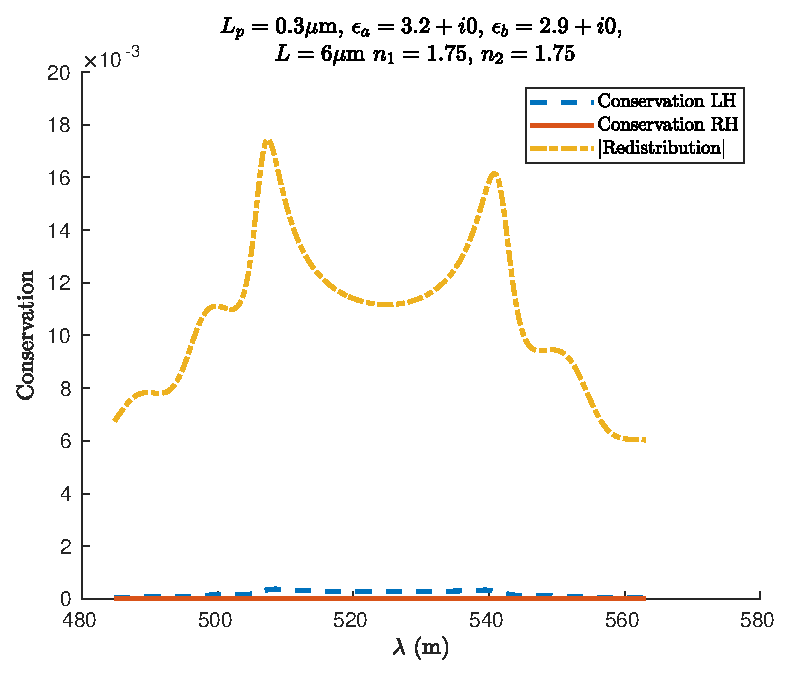
\includegraphics[width=\linewidth]{plots/simple/energy_cwt}
		\caption{}
		\label{fig:energy_cwt}
	\end{subfigure}
	\begin{subfigure}{0.49\linewidth}
		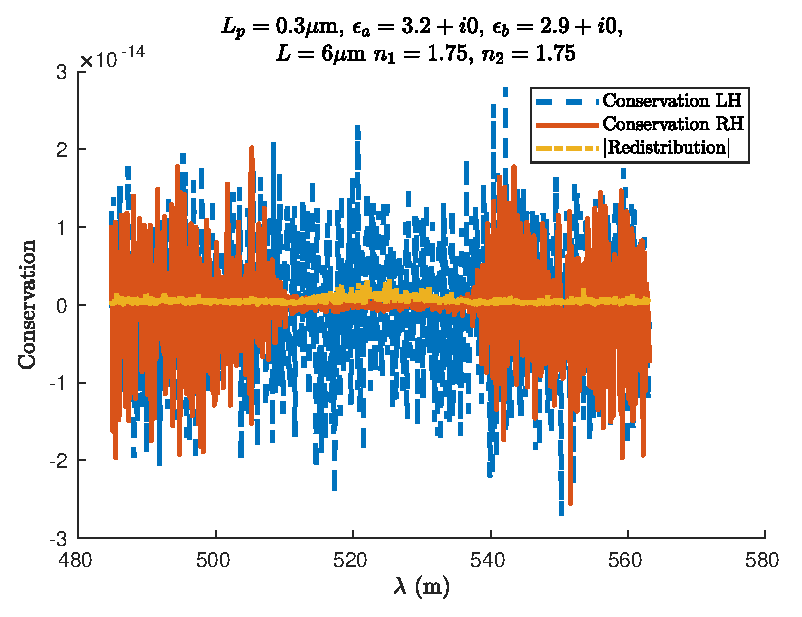
\includegraphics[width=\linewidth]{plots/simple/energy_oseen}
		\caption{}
		\label{fig:energy_oseen}
	\end{subfigure}
	\caption[Energy conservation in a simple cavity]{Energy conservation in a simple cavity. \ref{fig:energy_cwt} Coupled wave theory. \ref{fig:energy_oseen} Oseen method.}
	\label{fig:simple_cavity:energy_conservation}
\end{figure}

\subsection{Comparing laser action}

Equation \ref{eq:method:lasing_condition} is then compared to the result given by Topf and McCall\cite{topf_modes_2014}. The parameters used for the simulation are the same as in the original paper, and are reproduced in table \ref{tab:simple_cavity:simulation}. Figure \ref{fig:simple_cavity:surf} shows the invert of the determinant found using the approach described by Topf and McCall, developed CWT and exact theory. This shows that the implementation of coupled wave theory proposed here is coherent with previous results and exact theory.

\begin{table}
	\centering
	\begin{tabulary}{\linewidth}{LCC}
		\hline
		\hline
		Structural period of the chiral medium & $L_p$ & 300 nm \\
		Length of the chiral medium & $L$ & $20\times L_p$ \\
		Refractive index of the surrounding media & $n_1=n_2$ & 1 \\
		Average refractive index of the chiral medium (Re) & $\bar{n}$ & 1.7690 \\
		Detuning range & $\mathrm{Re}(\delta k L / 2)$ & $[0,12]$ \\
		Gain range & $-\mathrm{Im}(\delta k L / 2)$ & $[0,2.5]$ \\
		Coupling constant & $\kappa$ & $4/L$\\
		\hline
		\hline
	\end{tabulary}
	\caption[Parameters for the simple cavity]{Parameters used for simulation. Those are the same as in \cite{topf_modes_2014} to allow comparison of the found modes.}
	\label{tab:simple_cavity:simulation}
\end{table}

\begin{figure}
	\centering
	\begin{subfigure}{0.32\textwidth}
		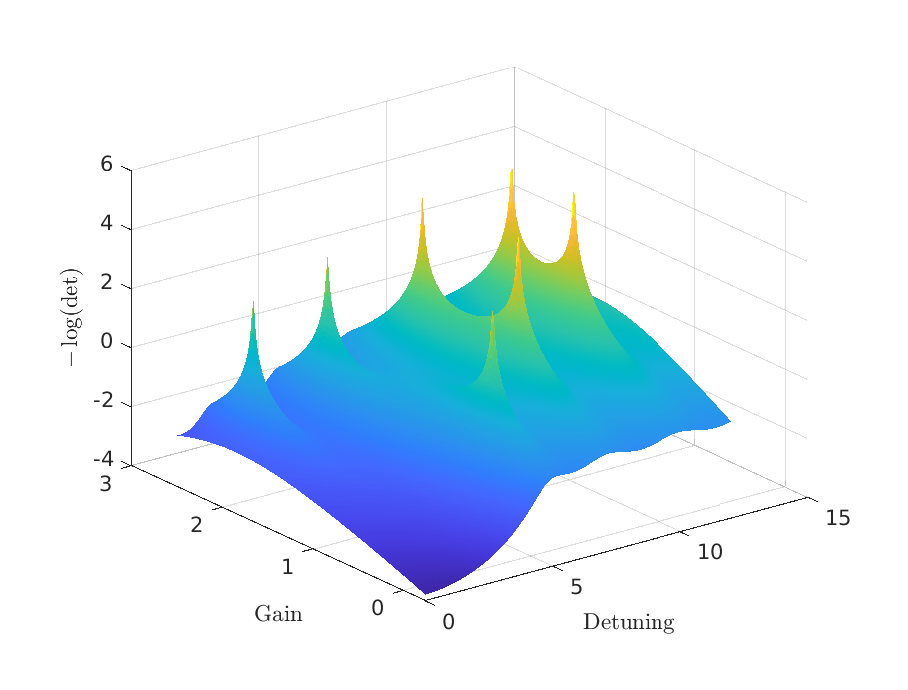
\includegraphics[width=\textwidth]{plots/simple/surface}
		\caption{}
		\label{fig:simple_cavity:mycwt_surf}
	\end{subfigure}
	\begin{subfigure}{0.32\textwidth}
		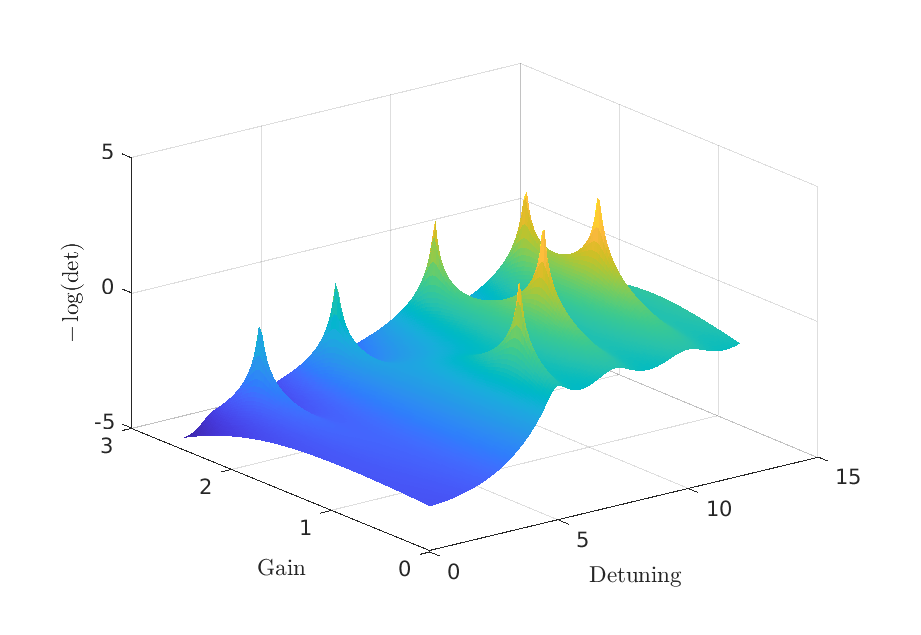
\includegraphics[width=\textwidth]{plots/simple/surface_topf}
		\caption{}
		\label{fig:simple_cavity:topf_surf}
	\end{subfigure}
	\begin{subfigure}{0.32\textwidth}
		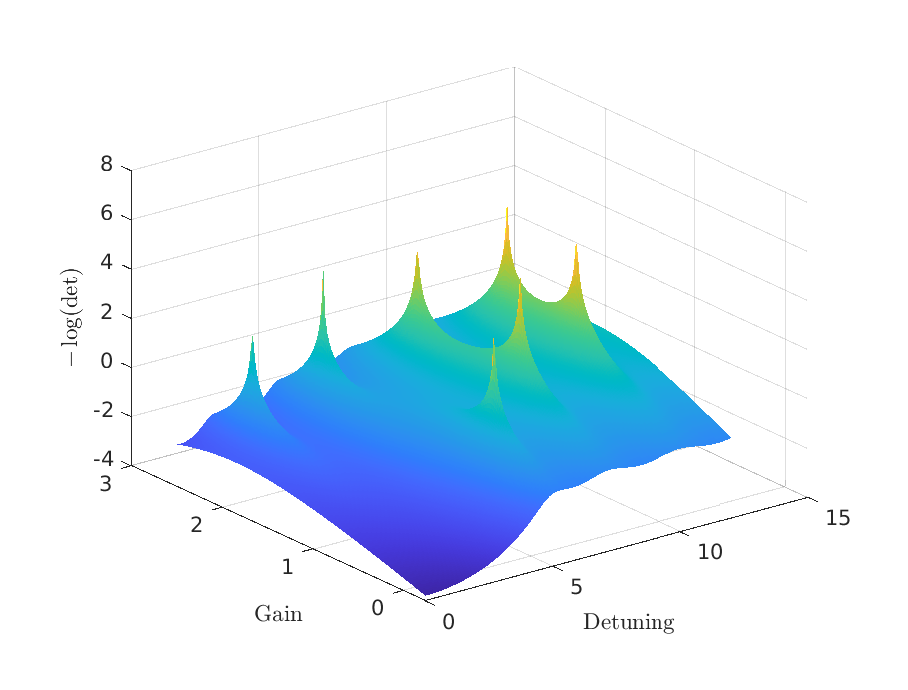
\includegraphics[width=\textwidth]{plots/simple/surface_oseen}
		\caption{}
		\label{fig:simple_cavity:oseen_surf}
	\end{subfigure}

	\begin{subfigure}{0.32\textwidth}
		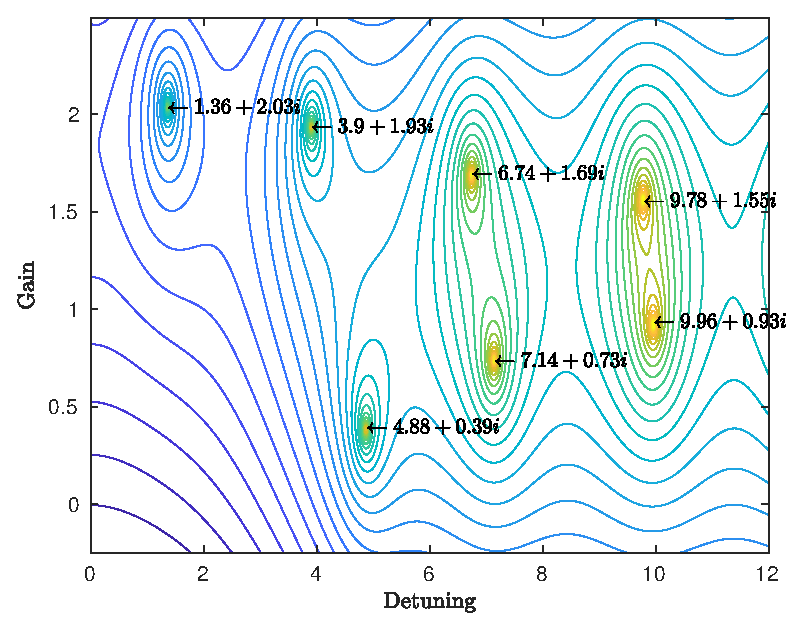
\includegraphics[width=\textwidth]{plots/simple/contour}
		\caption{}
		\label{fig:simple_cavity:mycwt_contour}
	\end{subfigure}
	\begin{subfigure}{0.32\textwidth}
		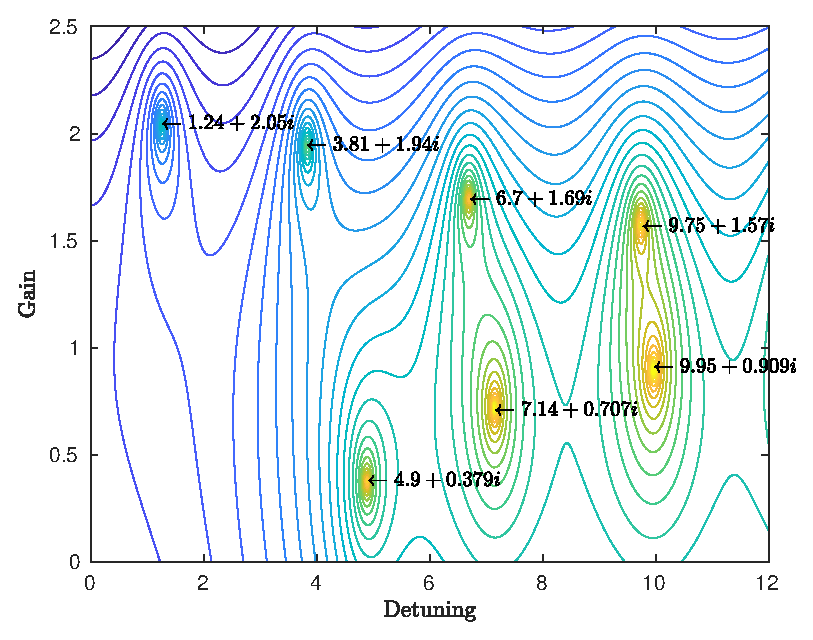
\includegraphics[width=\textwidth]{plots/simple/contour_topf}
		\caption{}
		\label{fig:simple_cavity:topf_contour}
	\end{subfigure}
	\begin{subfigure}{0.32\textwidth}
		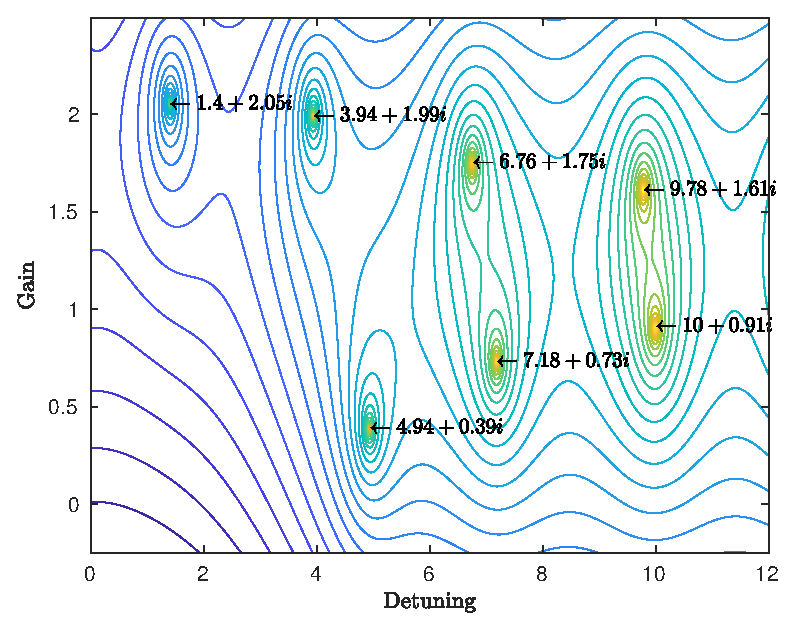
\includegraphics[width=\textwidth]{plots/simple/contour_oseen}
		\caption{}
		\label{fig:simple_cavity:oseen_contour}
	\end{subfigure}
	\caption[Comparison between methods for modeling a simple cavity.]{Comparison of the developed CWT and results reproduced from Topf and McCall\cite{topf_modes_2014}. \ref{fig:simple_cavity:mycwt_surf} shows the logarithm of the invert of the determinant of $\bm{M_{22}}$. \ref{fig:simple_cavity:mycwt_contour} is the corresponding contour plot where the lasing modes have been identified. \ref{fig:simple_cavity:topf_surf} is the invert of the determinant developed in \cite{topf_modes_2014} and \ref{fig:simple_cavity:topf_contour} is the corresponding contour plot. Finally \ref{fig:simple_cavity:oseen_surf} and \ref{fig:simple_cavity:oseen_contour} show the lasing coefficient obtained with the Oseen transformation.}
	\label{fig:simple_cavity:surf}
\end{figure}

Figure \ref{fig:simple_cavity:modes} shows the labelled output modes as well as the corresponding intensity distribution in the cavity. The first observation is that the overall intensity profile is, as expected, similar. The exact theory gives an account of the local variations in intensity due to the local variations of refractive index that are ignored in coupled wave theory. Moreover, coupled waves theory gives a good idea of the dynamics that take place in the cavity for each output mode. Indeed, for left-handed output polarisations, the intensity is mainly concentrated at the interfaces, corresponding to a Fabry-Pérot cavity where right-handed polarised light cannot propagate. On the other hand, for right-handed polarised light, Bragg reflections predominate.
\begin{figure}
	\centering
	\begin{subfigure}{.49\textwidth}
		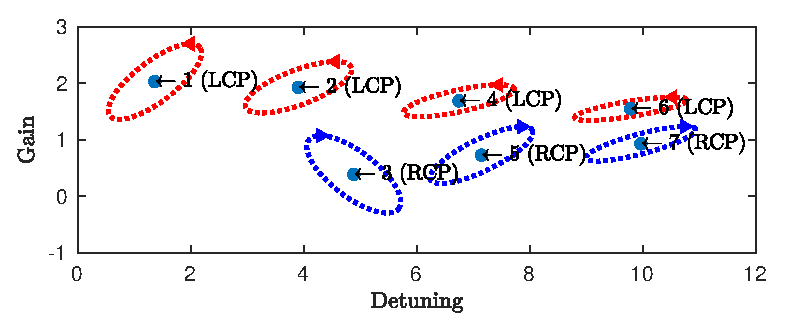
\includegraphics[width=\textwidth]{plots/simple/modes_found}
		\caption{Developed CWT}
		\label{fig:simple_cavity:modes_found}
	\end{subfigure}
	\begin{subfigure}{.49\textwidth}
		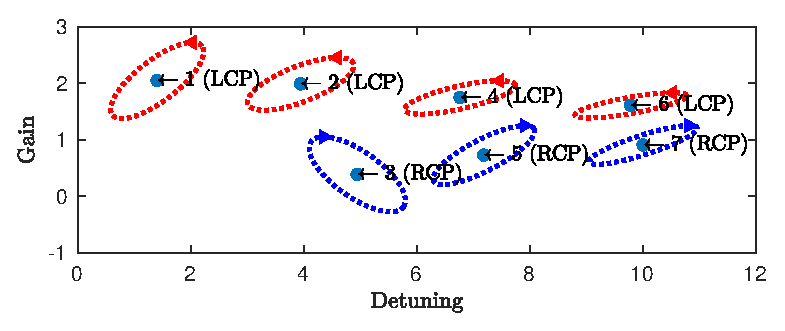
\includegraphics[width=\textwidth]{plots/simple/modes_found_oseen}
		\caption{Oseen method}
		\label{fig:simple_cavity:modes_found_oseen}
	\end{subfigure}
	\begin{subfigure}{.49\textwidth}
		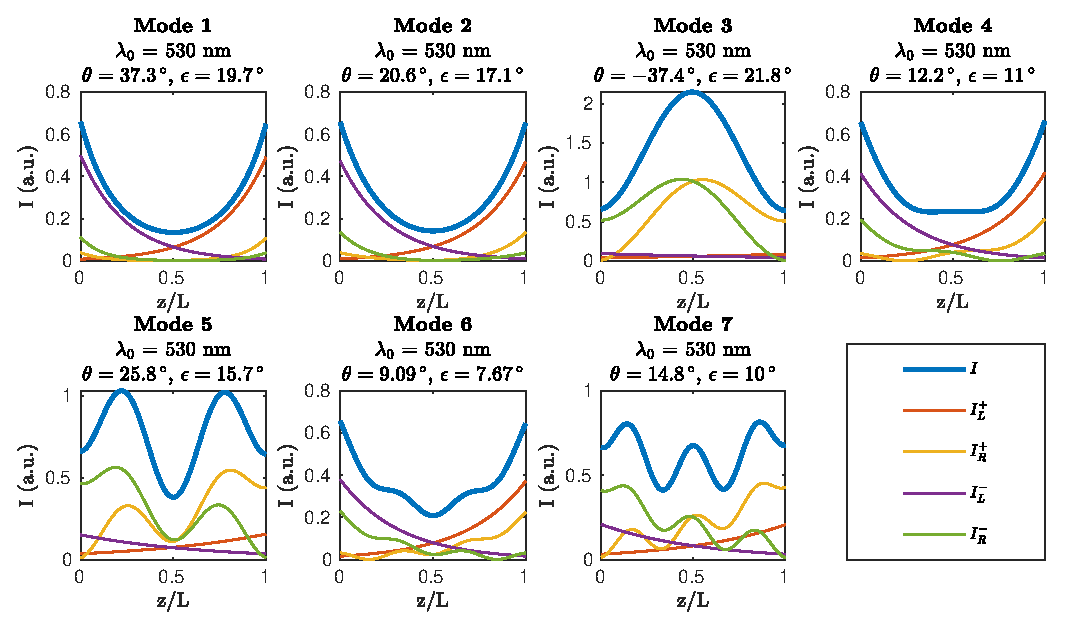
\includegraphics[width=\textwidth]{plots/simple/intensity_distribution}
		\caption{}
		\label{fig:simple_cavity:intensity_distribution}
	\end{subfigure}
	\begin{subfigure}{.49\textwidth}
		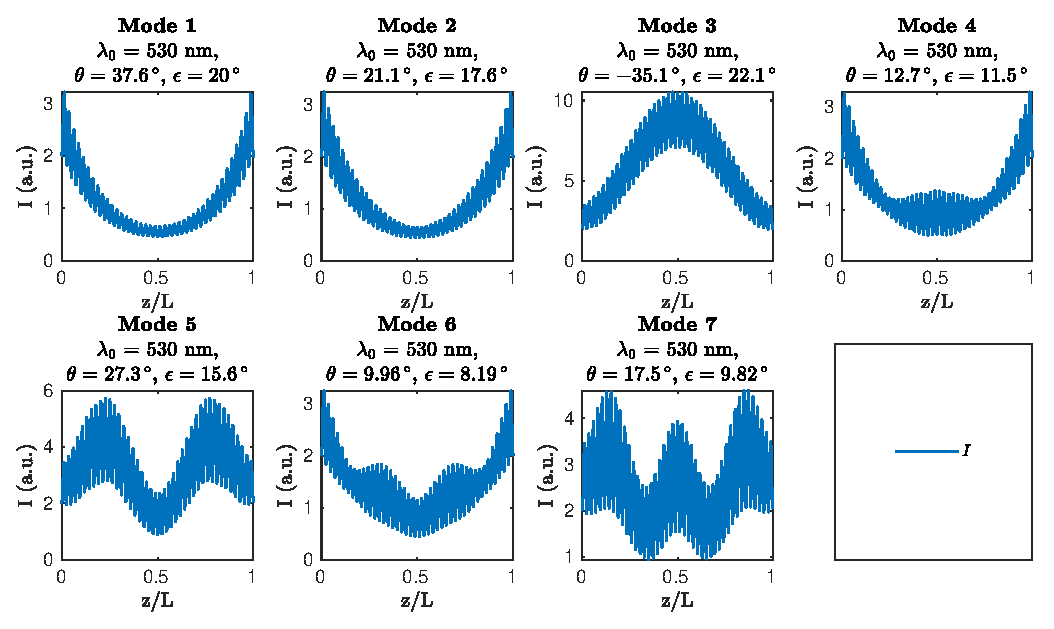
\includegraphics[width=\textwidth]{plots/simple/intensity_distribution_oseen}
		\caption{}
		\label{fig:simple_cavity:intensity_distribution_oseen}
	\end{subfigure}
	\caption[Comparison of intensity distribution for a simple cavity.]{\ref{fig:simple_cavity:modes_found} Labeled modes found with the developed CWT and corresponding output ellipses in medium 1. \ref{fig:simple_cavity:modes_found_oseen} Labeled modes found using exact theory and corresponding output ellipses. \ref{fig:simple_cavity:intensity_distribution} Intensity distribution in the cavity for the modes in \ref{fig:simple_cavity:modes_found}. \ref{fig:simple_cavity:intensity_distribution_oseen} Intensity distribution for modes given by exact theory.}
	\label{fig:simple_cavity:modes}
\end{figure}

\subsection{Conclusion on simple cavity}

This section mainly reproduced previous results, even though it introduced a comparison between coupled waves theory and exact theory that was not proposed before. Those results confirm that the implementation of both methods are fairly correct and increase the confidence in the new results proposed in the following sections, as they build on the same implementations.